\chapter{Proposed Method}
\label{chap:proposed_method}

\section{Problem Formulation}
\label{sec:method_problem}

Let \(y \in \mathbb{R}^{L}\) and \(x \in \mathbb{R}^{L}\) denote the noisy and clean speech waveforms, respectively. In single-channel speech enhancement, the noisy signal is modeled as
\begin{equation}
    y = x + n,
\end{equation}
where \(n\) denotes additive noise. Applying the short-time Fourier transform (STFT) gives noisy and clean complex spectra \(Y,X\in\mathbb{C}^{F\times T}\), where \(F\) and \(T\) denote frequency bins and time frames. The target of full-band speech enhancement is to estimate a clean full-band spectrum \(\hat{X}\) from the noisy full-band observation \(Y\), followed by inverse STFT reconstruction of the enhanced waveform \(\hat{x}\).

TF-Rehancer follows an observation-preserving filtering formulation. The neural network predicts a complex local time-frequency filter \(W\), and the final spectrum is obtained by applying this filter to a linear noisy STFT reference \(Y^{\mathrm{ref}}\):
\begin{equation}
    W = \mathcal{G}_{\theta}(\Phi(Y)), \qquad
    \hat{X} = W \otimes Y^{\mathrm{ref}}.
\end{equation}
Here, \(\mathcal{G}_{\theta}\) denotes TF-Rehancer, \(\Phi(Y)\) is the neural conditioning feature, and \(\otimes\) denotes local complex filtering over a time-frequency neighborhood. The compressed feature \(\Phi(Y)\) is used for conditioning, while the output operator is applied to the original linear noisy spectrum. Therefore, the model is not trained as an unconstrained direct generator of \(\hat{X}\); it estimates the filter coefficients used to transform the observed noisy spectrum.

For a 48 kHz full-band input, the upper band is already present in \(Y\), although it is corrupted by noise. TF-Rehancer treats this region as observed noisy evidence, derives decoder-side high-band query features from it, and refines the decoder representation before complex filtering.

\section{TF-Rehancer Architecture}
\label{sec:method_refinement_architecture}

This section describes TF-Rehancer as a low-band-guided full-band refinement pipeline: shared TF embedding, observed high-band query construction, cross-band decoder refinement, and full-resolution complex TF filtering.

\begin{figure}[!t]
    \centering
    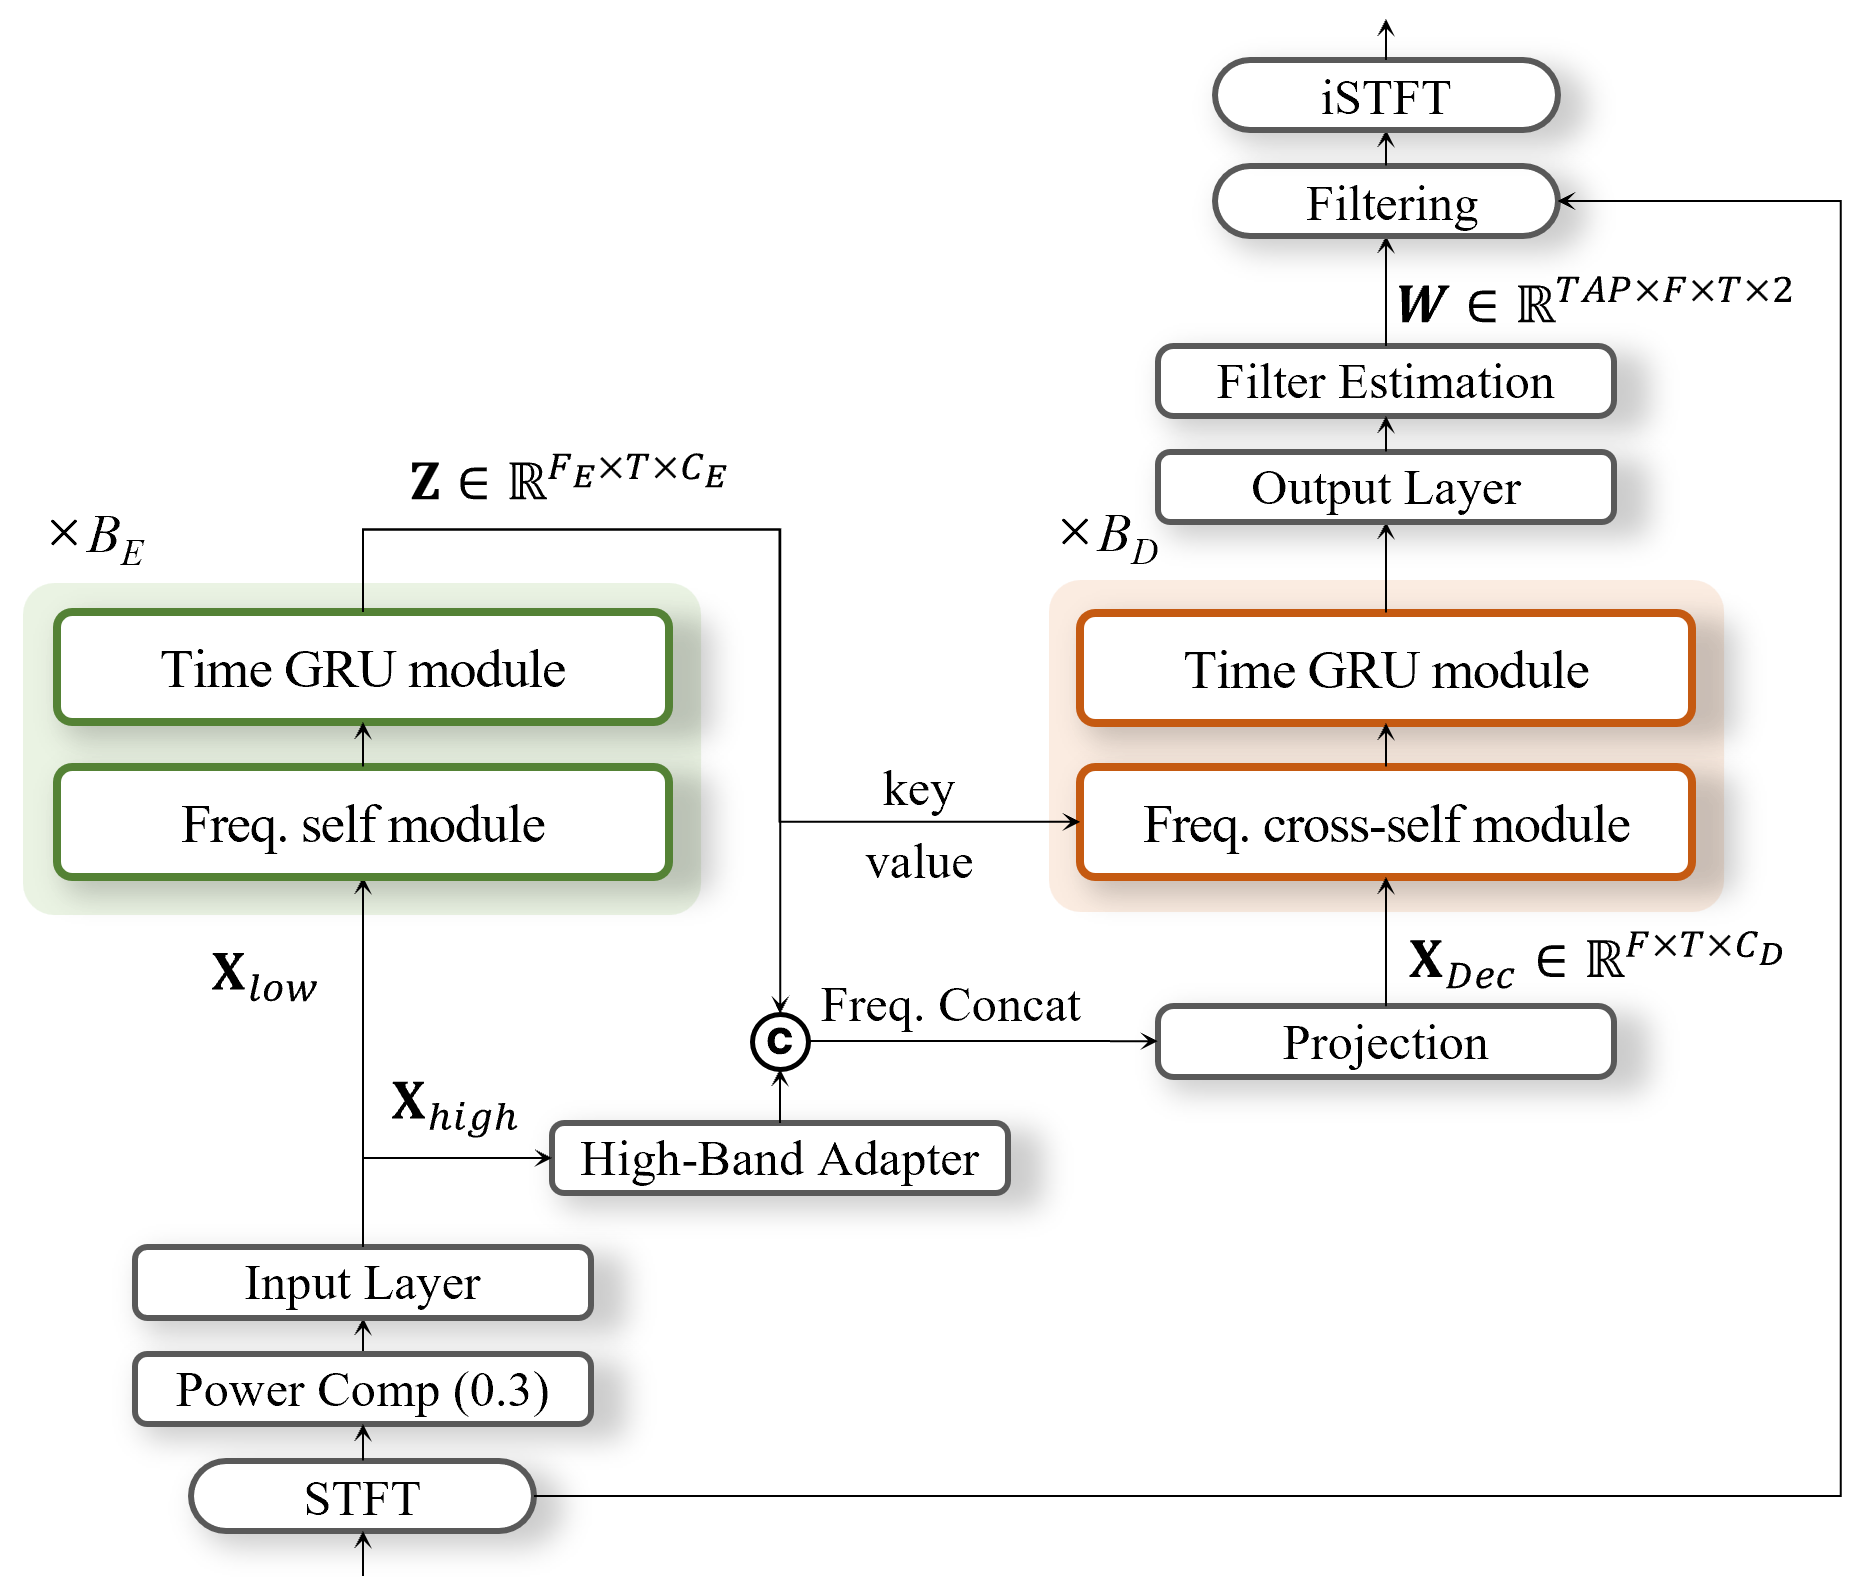
\includegraphics[width=0.92\textwidth]{figures/Architecture.png}
    \caption[Overall TF-Rehancer architecture]{Overall TF-Rehancer architecture. The shared input layer embeds the full-band STFT. The low-band region is encoded by the TF encoder, while the observed high-band region is carried as decoder-side query evidence. Decoder cross-attention updates the high-band tokens using low-band encoder context, and subsequent full-sequence decoder modeling produces features for complex TF filter estimation.}
    \label{fig:method_overall_flow}
\end{figure}

\subsection{SFI-STFT Conditioning and Shared Embedding}
\label{sec:method_architecture}

TF-Rehancer adopts the sampling-frequency-independent STFT (SFI-STFT) principle used in TF-Restormer~\cite{shin2026tfre}. The analysis window and hop are fixed by physical duration, 40 ms and 20 ms, rather than by a fixed sample count. Thus, the 16 kHz configuration uses \(N=640\), \(H=320\), and \(F=321\), while the 48 kHz configuration uses \(N=1920\), \(H=960\), and \(F=961\). This keeps the temporal frame geometry fixed across sampling rates and lets the frequency-bin count scale with bandwidth. Unlike TF-Restormer, which uses decoupled input-output rates for restoration and super-resolution, TF-Rehancer uses the same SFI-STFT parameterization for the noisy input, clean target, and inverse-STFT reconstruction in same-sampling-rate 16 kHz and 48 kHz speech enhancement settings.

Figure~\ref{fig:method_overall_flow} summarizes the TF-Rehancer architecture used in this thesis. The frontend constructs a power-law compressed conditioning feature while preserving a linear noisy STFT reference for the final filtering step. The shared input layer embeds the full-band STFT and reduces only the frequency resolution. A fixed 5 kHz split then routes low-band tokens to the TF encoder and observed high-band tokens to the decoder-side query path. The encoder uses four low-band time-frequency blocks to model speech-structure evidence. The decoder uses two cross-band time-frequency blocks that first update only the high-band decoder tokens using low-band key/value context and then model the full embedded sequence. Finally, FastFilterUpsample restores the original STFT frequency resolution, and the output layer estimates a local \(3\times3\) complex filter applied to \(Y^{\mathrm{ref}}\).

The neural conditioning feature is constructed from a power-law compressed complex STFT. Given \(\gamma=0.3\), the compressed spectrum and input feature are
\begin{equation}
    C_{\gamma}(Y)
    =
    Y\left(|Y|^2+\epsilon\right)^{(\gamma-1)/2},
    \qquad
    \Phi(Y)=
    \left[
    \operatorname{Re}(C_{\gamma}(Y)),
    \operatorname{Im}(C_{\gamma}(Y)),
    |C_{\gamma}(Y)|
    \right].
\end{equation}
Power-law compression stabilizes the dynamic range of spectral amplitudes for neural processing. The uncompressed noisy STFT reference \(Y^{\mathrm{ref}}\) is kept separately for the final filtering operation.

The feature \(\Phi(Y)\) is passed through a shared frequency-strided input stem, denoted by \(H=\operatorname{Stem}(\Phi(Y))\). The stem consists of \(\operatorname{Conv2D}(3 \rightarrow 48)\), batch normalization, and a SiLU activation. The convolution uses kernel size \((4,1)\), stride \((2,1)\), and padding \((2,0)\), so it reduces only the frequency resolution and preserves the frame rate. This shared stem is used for both 16 kHz and 48 kHz configurations. After the stem, the embedded frequency resolution is \(F_{\mathrm{emb}}=161\) at 16 kHz and \(F_{\mathrm{emb}}=481\) at 48 kHz. The shared stem compresses the frequency axis for efficient modeling while deriving high-band decoder tokens from the observed high-band portion of the input representation.

On the output side, the decoder representation is restored to the original STFT frequency resolution before estimating local complex filter coefficients. Thus, both input-side embedding and output-side filtering are described as local convolutional transformations around an explicit STFT reference, rather than as unconstrained waveform generation.

\subsection{Observed High-Band Query Construction}
\label{sec:method_query_refinement}

\begin{center}
    \centering
    \begin{tabular}{@{}c@{\hspace{0.055\textwidth}}c@{\hspace{0.055\textwidth}}c@{}}
        \raisebox{-0.01\textheight}{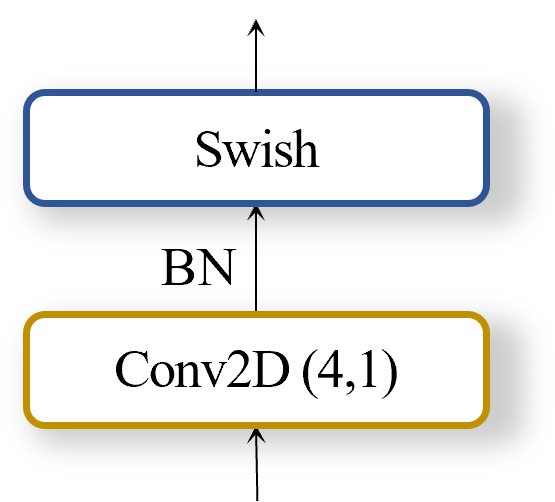
\includegraphics[width=0.245\textwidth]{figures/Input_Layer.png}} &
        \raisebox{-0.02\textheight}{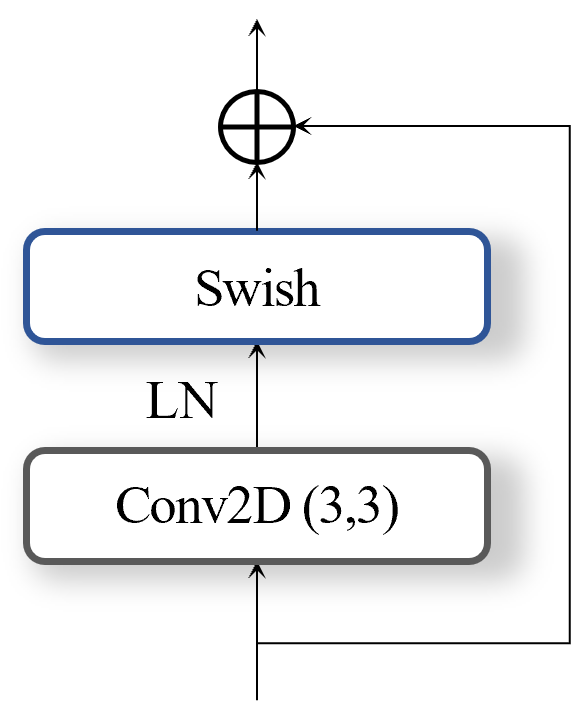
\includegraphics[width=0.245\textwidth]{figures/HighBandRefine_block.png}} &
        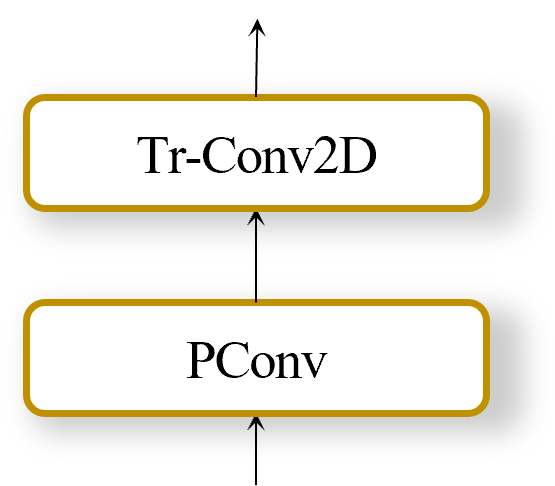
\includegraphics[width=0.245\textwidth]{figures/Output_Layer.png} \\
        {\footnotesize (a) Input Layer} &
        {\footnotesize (b) High-Band Adapter} &
        {\footnotesize (c) Output Layer}
    \end{tabular}
    \captionof{figure}[Local convolutional layer notation]{Local convolutional layer notation used for the input stem, high-band adapter, and output-side upsampling/filtering layers. The channel width, stride, and normalization differ by module and are specified in the text.}
    \label{fig:method_io_hbr_layer}
\end{center}

After the shared stem, TF-Rehancer splits the embedded frequency axis using a 5 kHz cutoff into \(H_{\mathrm{low}}\) and \(H_{\mathrm{high}}\). At 16 kHz, this gives \(F_{\mathrm{low}}=101\) and \(F_{\mathrm{high}}=60\). At 48 kHz, it gives \(F_{\mathrm{low}}=101\) and \(F_{\mathrm{high}}=380\). Thus, the same low-band speech-structure region is encoded at both sampling rates, while the 48 kHz model keeps a much larger observed high-band region in the decoder path.

The high-band branch is derived from the observed high-band stem feature:
\begin{equation}
    Q_h = H_{\mathrm{high}} + \operatorname{Adapter}_{h}(H_{\mathrm{high}}).
\end{equation}
The adapter is a residual local convolutional block with SiLU activation and layer normalization, using the local convolutional layer notation summarized in Fig.~\ref{fig:method_io_hbr_layer}. This block aligns the observed high-band representation with the decoder query space before cross-band refinement. It does not perform decoder refinement by itself; it prepares the high-band tokens for the decoder. The query source remains the observed high-band embedding, and the adapter only provides a lightweight local transformation before cross-band refinement.

We next describe the low-band encoder that produces the context representation used by the decoder cross-attention. The low-band encoder maps \(H_{\mathrm{low}}\) to an encoded representation \(Z\) using four stacked blocks. Each block combines frequency feed-forward layers, frequency-axis self-attention with RoPE, and FastGRU2 temporal modeling. The encoder does not use a frequency projection layer or a pre-encoder sinusoidal positional encoding. Its role is to model speech structure from the low-band region, where harmonic and formant-related evidence is relatively dense.

The encoder frequency module follows a Macaron-style structure: a convolutional feed-forward layer is placed before and after frequency-axis self-attention. This F-ConvFFN--F-MHSA--F-ConvFFN ordering lets local convolutional mixing and global frequency attention complement each other. The decoder frequency module extends this pattern by inserting cross-attention before full-sequence self-attention, i.e., F-MHCA--F-MHSA--F-ConvFFN.

RoPE is applied to frequency-axis attention to encode the relative order of frequency tokens without relying on a learned absolute positional table. This is useful because the frequency axis has a fixed physical ordering, while the number of tokens differs between 16 kHz and 48 kHz settings. In decoder cross-attention, the high-band query and low-band key/value tokens occupy different frequency regions, so RoPE offsets preserve their relative frequency positions during cross-band attention.

To reduce the cost of the frequency feed-forward layers, TF-Rehancer uses an efficient convolutional FFN. Instead of applying a large convolutional FFN over the full frequency sequence, the module first downsamples the frequency-axis sequence by adaptive average pooling. It then applies grouped gated 1-D convolutions on the shortened sequence, using separate value and gate branches followed by SiLU gating. We use group convolution with two groups to reduce computation. The output is projected back, upsampled to the original frequency length, and added as a scaled residual correction. This design keeps a full-length residual path while applying the expensive gated convolutional correction on a shorter sequence.

\subsection{Cross-Band Decoder Refinement}
\label{sec:method_decoder_refinement}

\begin{center}
    \centering
    \begin{tabular}{@{}c@{\hspace{0.025\textwidth}}c@{\hspace{0.025\textwidth}}c@{}}
        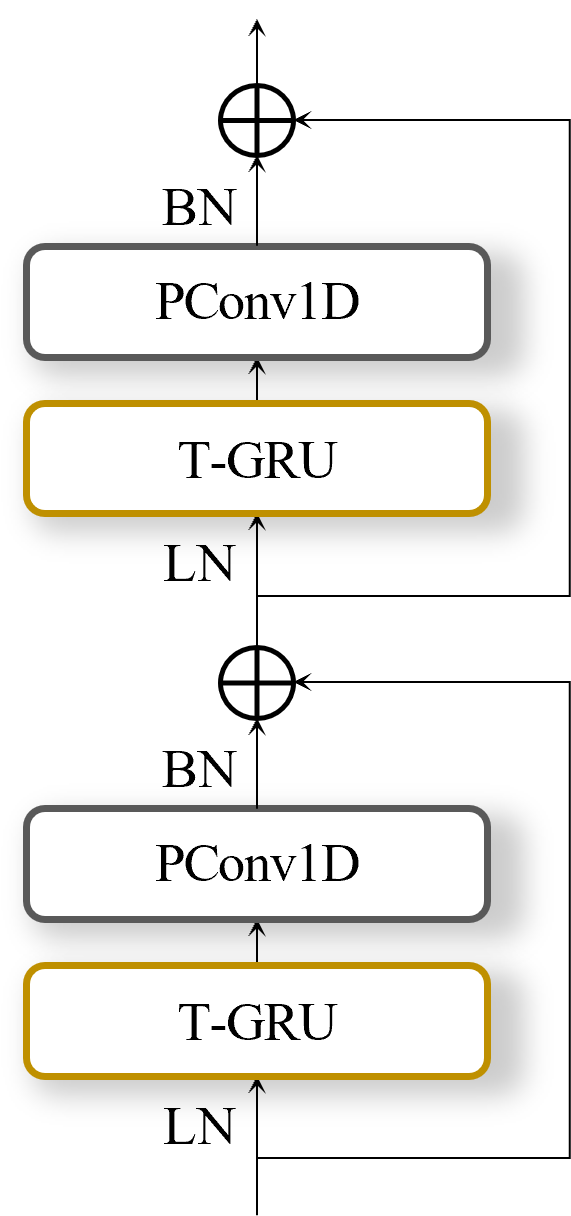
\includegraphics[width=0.2\textwidth]{figures/Time_GRU_module.png} &
        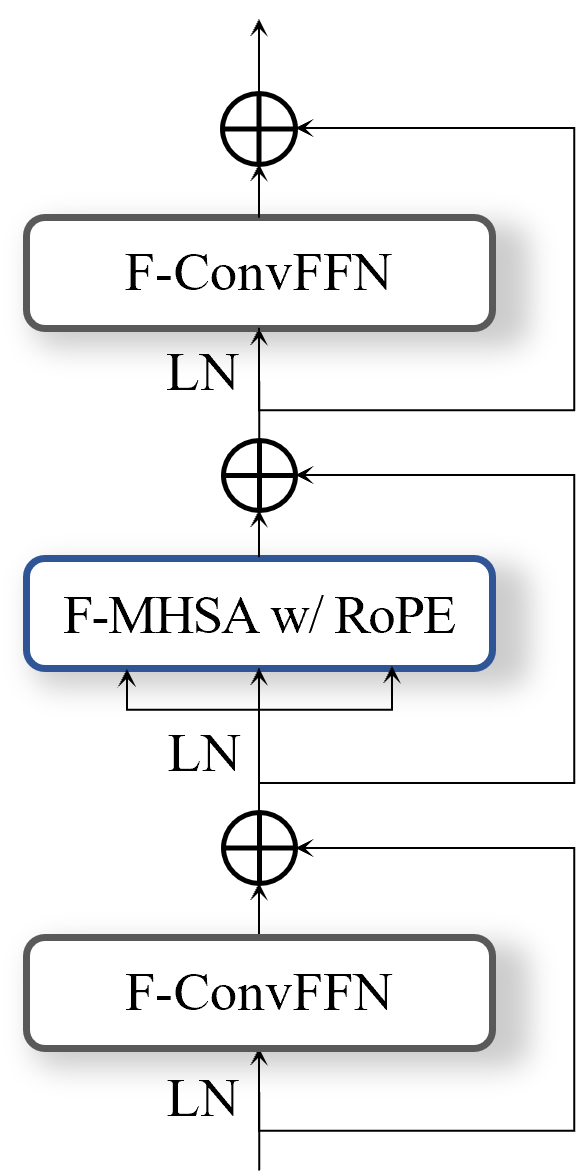
\includegraphics[width=0.21\textwidth]{figures/Freq_self_module.png} &
        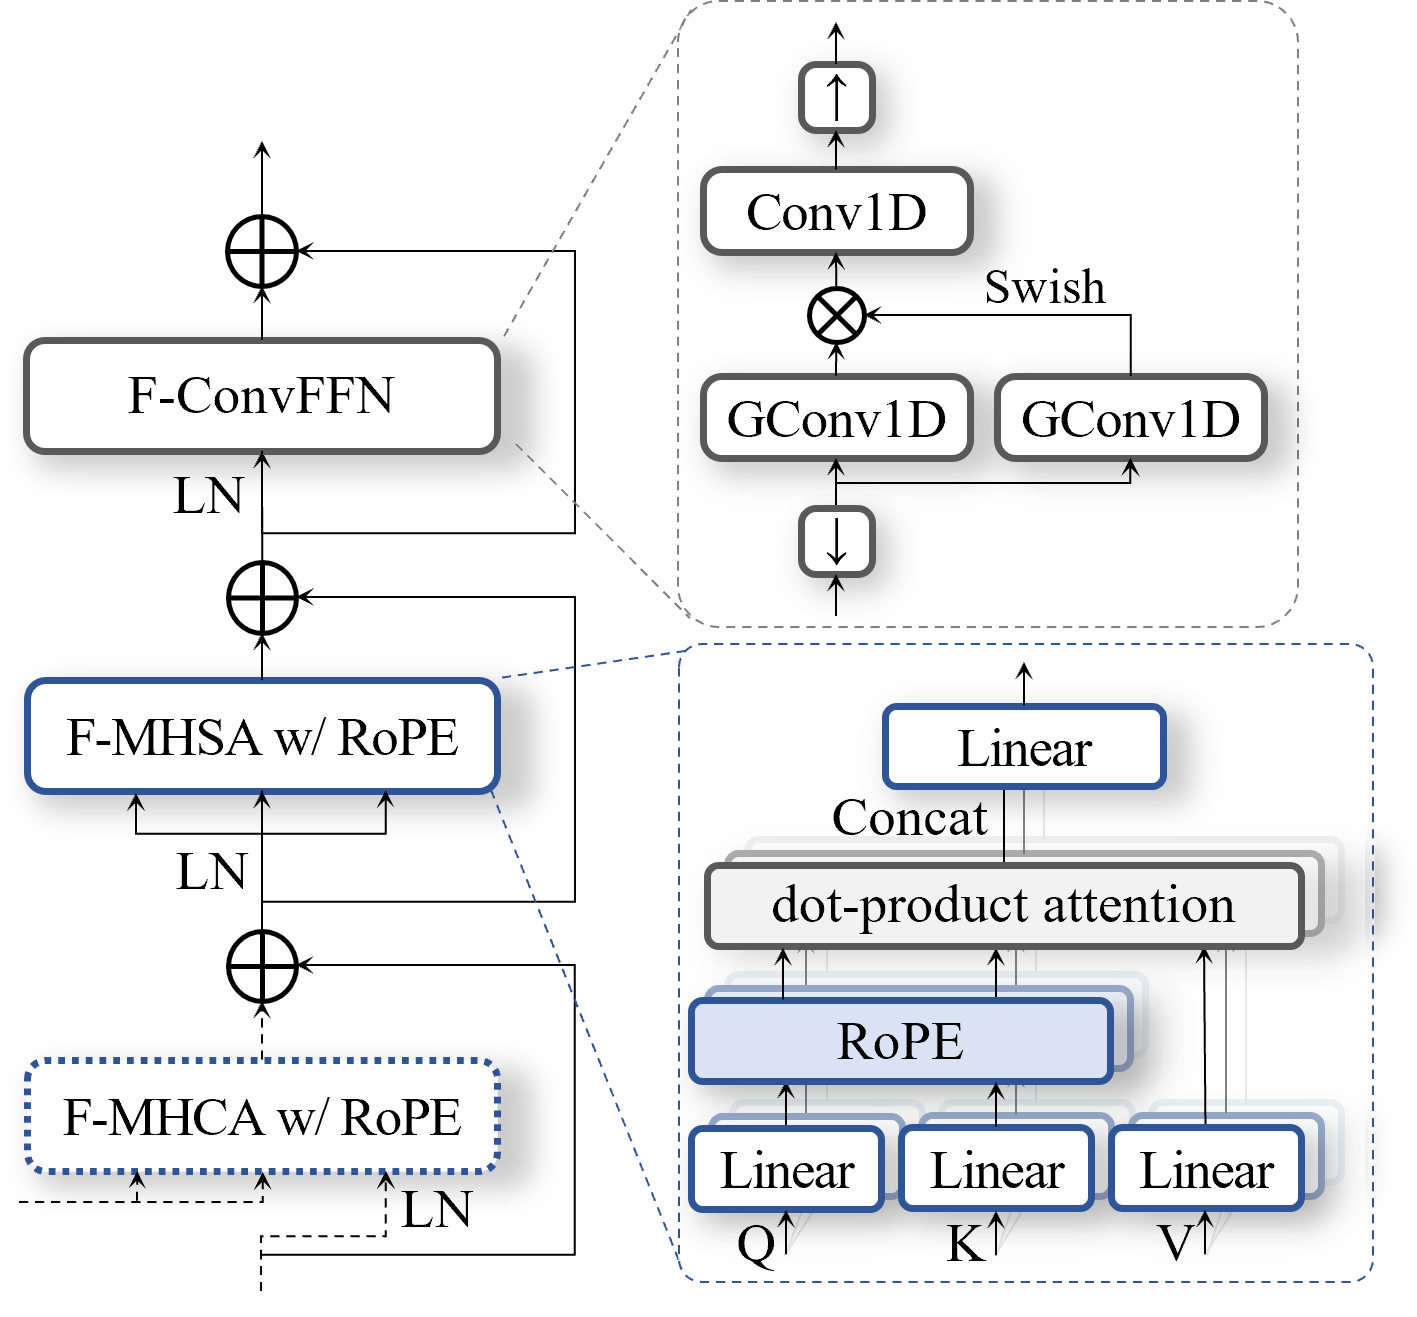
\includegraphics[width=0.51\textwidth]{figures/Freq_cross_self_module.png} \\
        {\footnotesize (a) Time GRU Module} &
        {\footnotesize (b) Freq. Self Module} &
        {\footnotesize (c) Freq. Cross-Self Module}
    \end{tabular}
    \captionof{figure}[TF-Rehancer encoder and decoder core blocks]{TF-Rehancer encoder and decoder core blocks. The encoder frequency module uses a Macaron-style F-ConvFFN--F-MHSA--F-ConvFFN structure with RoPE. The decoder frequency module first applies F-MHCA to update high-band tokens using low-band encoder context, then applies full-sequence F-MHSA and F-ConvFFN.}
    \label{fig:method_core_blocks}
\end{center}

The decoder first forms a full embedded sequence by concatenating the low-band encoder output \(Z\) and the adapted high-band query \(Q_h\) along the frequency axis. A linear projection with layer normalization maps the concatenated 48-channel representation to the 24-channel decoder width. This projection is a separate alignment stage between the encoder/query interface and the decoder blocks.

Let the projected decoder input be split as \(D=[D_{\mathrm{low}};D_{\mathrm{high}}]\), where \(D_{\mathrm{high}}\) corresponds to the observed high-band portion. TF-Rehancer uses two decoder blocks. In each block, \(D_{\mathrm{low}}\) passes through the cross-attention stage without being updated by MHCA, while \(D_{\mathrm{high}}\) is used as the query. The key and value are obtained from the low-band encoder output \(Z\):
\begin{equation}
    Q = \Pi_q(D_{\mathrm{high}}), \qquad
    K = \Pi_k(Z), \qquad
    V = \Pi_v(Z).
\end{equation}
The high-band update is then computed as
\begin{equation}
    \tilde{D}_{\mathrm{high}}
    =
    D_{\mathrm{high}}
    +
    \operatorname{MHCA}(Q,K,V),
\end{equation}
and the decoder sequence is reconstructed as
\begin{equation}
    \tilde{D}=[D_{\mathrm{low}};\tilde{D}_{\mathrm{high}}].
\end{equation}
The projection operators \(\Pi_q\), \(\Pi_k\), and \(\Pi_v\) are implemented inside the MHCA module, so the input widths of the decoder-side query and low-band context need not be identical. Cross-attention therefore performs directed low-to-high conditioning by updating only the observed high-band decoder tokens. The following frequency self-attention, frequency feed-forward processing, and FastGRU2 temporal modeling operate on \(\tilde{D}\), so low- and high-band tokens interact over the full embedded sequence after the directed update.

This design separates three roles. The high-band adapter prepares observed high-band query evidence from \(H_{\mathrm{high}}\). The concat-projection layer aligns the low-band encoder output and high-band query into the decoder width. The decoder blocks then perform cross-attention-based high-band token update followed by full-sequence time-frequency modeling.

\subsection{Complex TF Filtering}
\label{sec:method_filtering}

\begin{center}
    \centering
    \begin{tabular}{@{}c@{\hspace{0.05\textwidth}}c@{}}
        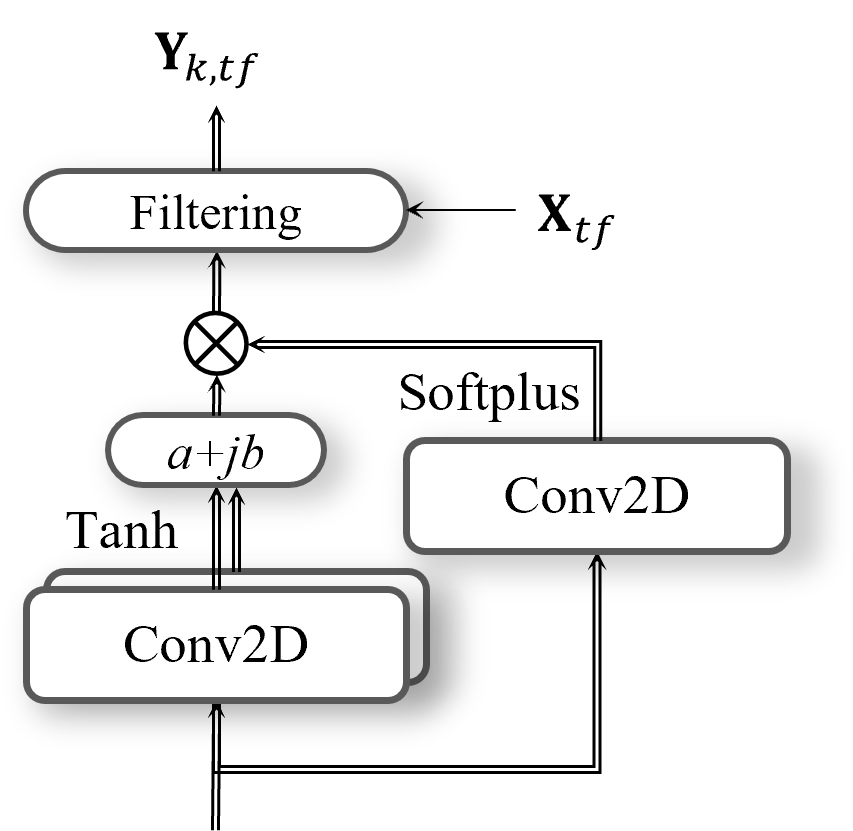
\includegraphics[width=0.30\textwidth]{figures/Filtering_Module.png} &
        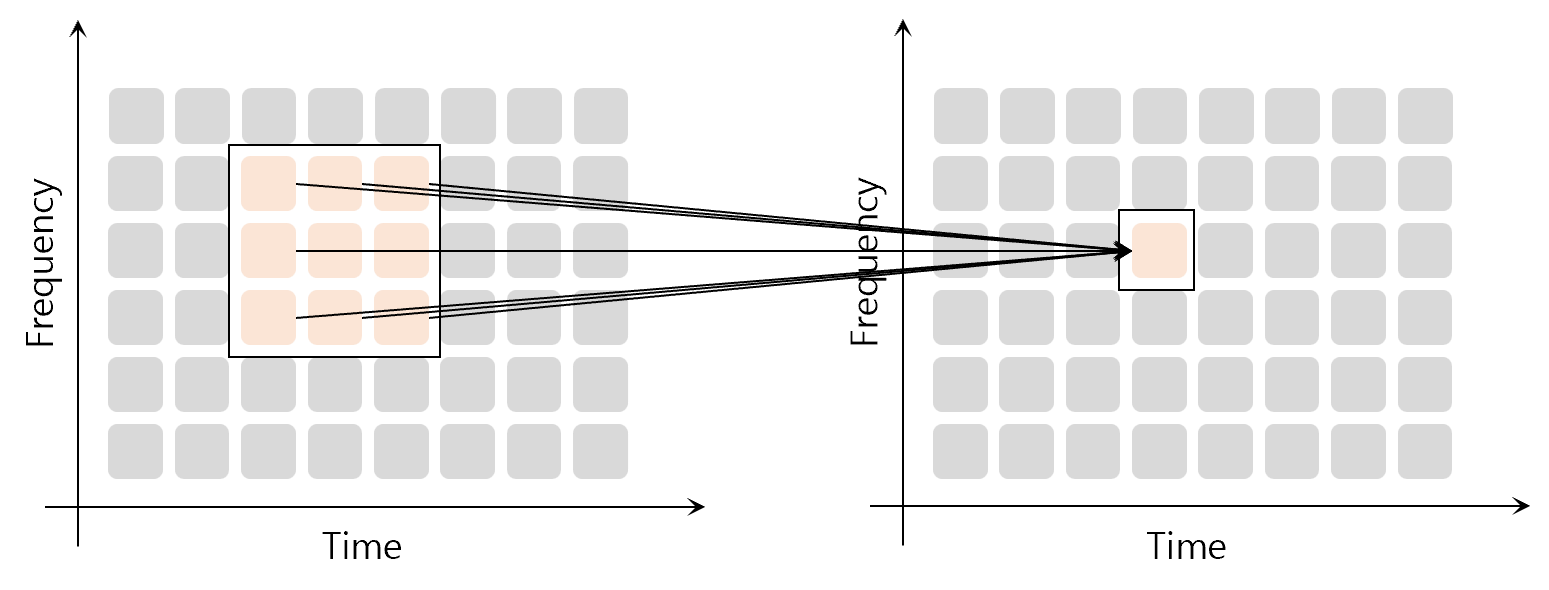
\includegraphics[width=0.62\textwidth]{figures/3x3DeepFiltering_Demonstration.png} \\
        {\footnotesize (a) Filtering Module} &
        {\footnotesize (b) Local \(3\times3\) Complex TF Filtering}
    \end{tabular}
    \captionof{figure}[Complex TF filtering module]{Complex TF filtering module. TF-Rehancer predicts complex filter coefficients and applies them to a local time-frequency neighborhood of the noisy STFT reference.}
    \label{fig:method_deep_filtering}
\end{center}

The decoder output is still at embedded frequency resolution. Before filter estimation, TF-Rehancer restores it to the original STFT frequency resolution using FastFilterUpsample. This module uses a pointwise convolution followed by transposed convolution along the frequency axis. The restored full-resolution feature is then passed to a partial-convolution filter head and a local \(3 \times 3\) time-frequency convolution.
The output-side convolutional operations follow the compact local-layer notation in Fig.~\ref{fig:method_io_hbr_layer}, while the explicit filtering operation is described below.

For each time-frequency bin, the head predicts nine complex taps over the local offsets \(\Delta f,\Delta t\in\{-1,0,1\}\). The raw head output has 27 channels: one magnitude scale, one real component, and one imaginary component for each tap. A softplus activation constrains the magnitude scale to be positive, and tanh activations bound the real and imaginary components before forming the complex coefficients \(W_{\Delta f,\Delta t,f,t}\).
The enhanced spectrum is computed as
\begin{equation}
    \hat{X}_{f,t}
    =
    \sum_{\Delta f=-1}^{1}
    \sum_{\Delta t=-1}^{1}
    W_{\Delta f,\Delta t,f,t}
    Y^{\mathrm{ref}}_{f+\Delta f,t+\Delta t}.
\end{equation}
Boundary positions are padded before local neighborhoods are gathered. This operation is a complex filtering operation, not a correlation estimate. The coefficients \(W\) are the predicted filter weights used to construct \(\hat{X}\); they are conditioned on the decoder feature and applied to the observed noisy STFT reference.

The filtering head is therefore the output estimator of the proposed refinement architecture, while the main representation-level contribution lies in low-band-guided full-band refinement.

\section{Training Objective}
\label{sec:method_training}

TF-Rehancer is trained with a composite enhancement loss using the same \(\gamma=0.3\) power-law compression as the input feature, with an \(\epsilon\)-stabilized magnitude. Let \(\hat{X}\) and \(X\) denote the estimated and clean complex STFTs, and let \(\hat{x}=\operatorname{iSTFT}(\hat{X})\) and \(x=\operatorname{iSTFT}(X)\) denote the corresponding waveforms. The total enhancement loss is
\begin{equation}
    \mathcal{L}
    =
    \lambda_{\mathrm{mag}}\mathcal{L}_{\mathrm{mag}}
    +
    \lambda_{\mathrm{cplx}}\mathcal{L}_{\mathrm{cplx}}
    +
    \lambda_{\mathrm{cons}}\mathcal{L}_{\mathrm{cons}}
    +
    \lambda_{\mathrm{wav}}\mathcal{L}_{\mathrm{wav}}
    +
    \lambda_{\mathrm{pesq}}\mathcal{L}_{\mathrm{pesq}}.
\end{equation}
Using \(C_\gamma(\cdot)\) for the compressed complex spectrum and \(\operatorname{RI}(\cdot)\) for real-imaginary channel stacking, the spectral terms are
\begin{align}
    \mathcal{L}_{\mathrm{mag}}
    &=
    \operatorname{MSE}
    \left(
    |C_\gamma(\hat{X})|,
    |C_\gamma(X)|
    \right),
    \\
    \mathcal{L}_{\mathrm{cplx}}
    &=
    \operatorname{MSE}
    \left(
    \operatorname{RI}(C_\gamma(\hat{X})),
    \operatorname{RI}(C_\gamma(X))
    \right).
\end{align}
\(\mathcal{L}_{\mathrm{mag}}\) matches the compressed magnitude envelope and encourages energy consistency across frequency bands, including the upper band. It does not directly supervise phase. \(\mathcal{L}_{\mathrm{cplx}}\) compares the compressed real and imaginary components, so it gives phase-sensitive supervision for the complex filter output.

The consistency term is computed after waveform reconstruction:
\begin{equation}
    \tilde{X}
    =
    \operatorname{STFT}
    \left(
    \operatorname{iSTFT}(\hat{X})
    \right),
    \qquad
    \mathcal{L}_{\mathrm{cons}}
    =
    \operatorname{MSE}
    \left(
    \operatorname{RI}(C_\gamma(\tilde{X})),
    \operatorname{RI}(C_\gamma(X))
    \right).
\end{equation}
Thus, \(\mathcal{L}_{\mathrm{cons}}\) does not merely compare two pre-reconstruction STFT tensors. It penalizes spectra that appear plausible before inverse STFT but become inconsistent after the waveform is reconstructed and transformed back to the STFT domain.

The waveform and perceptual auxiliary terms are
\begin{equation}
    \mathcal{L}_{\mathrm{wav}}
    =
    \|\hat{x}-x\|_{1},
    \qquad
    \mathcal{L}_{\mathrm{pesq}}
    =
    \operatorname{PesqLoss}
    \left(
    \mathcal{R}_{16}(\hat{x}),
    \mathcal{R}_{16}(x)
    \right),
\end{equation}
where \(\mathcal{R}_{16}\) denotes resampling to 16 kHz when the training waveform is 48 kHz and the identity operation for 16 kHz training. \(\mathcal{L}_{\mathrm{wav}}\) reduces sample-level reconstruction error and time-domain artifacts that may not be fully captured by spectral losses. \(\mathcal{L}_{\mathrm{pesq}}\) is a differentiable PESQ-like training loss, not the reported evaluation PESQ score, and is used only as a weak perceptual regularizer.

The loss weights for \(\mathcal{L}_{\mathrm{mag}}\), \(\mathcal{L}_{\mathrm{cplx}}\), \(\mathcal{L}_{\mathrm{cons}}\), \(\mathcal{L}_{\mathrm{wav}}\), and \(\mathcal{L}_{\mathrm{pesq}}\) are \(0.3\), \(0.2\), \(0.3\), \(0.2\), and \(0.001\), respectively. Therefore, optimization is driven mainly by compressed spectral reconstruction, reconstruction consistency, and waveform-domain supervision, while the PESQ term remains lightly weighted.
